\setcounter{section}{0} 

\part{Probabilités}

\section{Ensembles finis}

\subsection{Définitions}

\begin{itemize}
\item[*] Soit $E$ un ensemble. \\ $E$ est un ensemble fini si et seulement si $E$ est vide, ou si E est constitué d'un nombre défini d'éléments.
\item[*] Soit E un ensemble fini non vide. On appelle \underline{cardinal de E} et on note $\mathrm{Card} \; E$ le nombre d'éléments de E.
\end{itemize} 

\vspace*{.3cm}

\textbf{Exemple}

\centerline{\begin{tabular}{c@{$\qquad \qquad$}c}
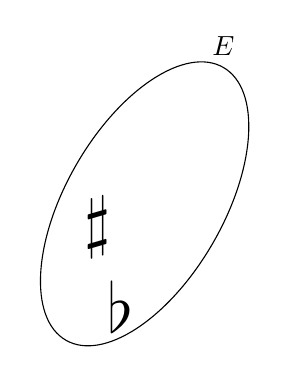
\begin{tikzpicture}
% \draw [help lines] (-2,-2) grid (2,2)  ;
% \tkzTabInit[help]
{\begin{scope} [rotate=-30]
\draw (0,0)  circle  (1 and 2); 
% \draw (0,0) ++(0:-.2) circle (.6 and 1); 
\end{scope} 
\draw (1,2) node {$E$} ; 
\draw (.2,.9) node {\Large $\bigstar$} ; 
\draw (.3,-.1) node { \Large $\blacksquare$} ; 
\draw (-.6,-.3) node { \Huge $\sharp$} ; 
\draw (-.3,-1.3) node {\Huge $\flat$} ; 
}
\end{tikzpicture} 
                     &    \raisebox{8ex}{Card E = 4} \\
                     & \\
\end{tabular}} 

On complète la définition en posant : $\mathrm{Card} \; \varnothing = 0 $.

\subsection{Propriétés}

Soient E et F deux ensembles finis.

\textbf{a)} 


\centerline{
\begin{tabular}{c@{$\qquad \qquad$}c}
                       & \\
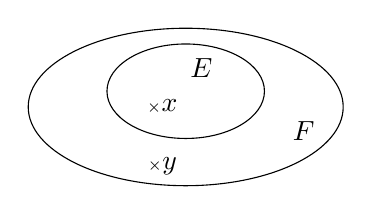
\begin{tikzpicture}
% \draw [help lines] (-2,-2) grid (2,2)  ;
\begin{scope}   [rotate=-90]
\draw (0,0)  circle  (1 and 2); 
\draw (0,0) ++(0:-.2) circle (.6 and 1); 
\end{scope} 
\draw (1.5,-0.3) node {$F$} ; 
\draw (.2,.5) node {$E$} ; 
\draw (-.3,0) node {{\tiny $\times$} $\!\!x$} ; 
\draw (-.3,-.75) node {{\tiny $\times$} $\!\!y$} ; 
\end{tikzpicture}
                     &    \raisebox{5ex}{\parbox{5cm}{
                               \begin{itemize}
                                  \item[*] $\forall x\in E$, $x\in F$.
                                  \item[*] $\exists y\in F$ tel que $y\notin E$                               
                               \end{itemize} 
                               \bigskip                            
                               Si $E\subset F$, alors Card $E \leq$ Card $F$.
                               }} \\
                      & \\         
\end{tabular}} 


\textbf{b)} 

%Dessin, et à côté le texte ci-dessous.

\begin{center}

\begin{tabular}{c@{$\qquad \qquad$}c}
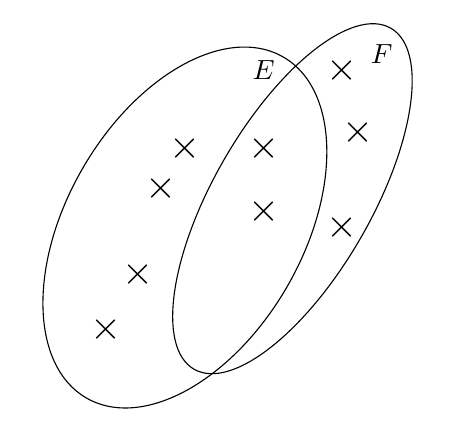
\begin{tikzpicture}
% \draw [help lines] (-2,-2) grid (3,3)  ;

\begin{scope} [rotate=-30]
    \draw (0,0) circle (1.5 and 2.5); 
    \draw (1,1) circle (1   and 2.5); 
\end{scope} 

\draw (1,2) node {$E$} ; 
\draw (2.5,2.2) node {$F$} ; 

\draw (-1,.-1.3)  node {\Large $\times$} ; 
\draw (-.6,-.6)   node {\Large $\times$} ; 
\draw (-.3,.5)    node {\Large $\times$} ; 
\draw (1,.2) node {\Large $\times$} ; 
\draw (1,1)   node {\Large $\times$} ; 
\draw (0,1)   node {\Large $\times$} ; 
% \draw (.8,1)   node {\Large $\times$} ; 
\draw (2,0)   node {\Large $\times$} ; 
\draw (2.2,1.2)   node {\Large $\times$} ; 
\draw (2,2) node {\Large $\times$} ; 
\end{tikzpicture} 
                     &    \raisebox{15ex}{\parbox{7cm}{
                               On a : $\mathrm{Card} \; E = 6 \qquad $ et $\qquad \mathrm{Card} \; F = 5$.\\
                            
                            \bigskip

                              Card $\left(E \cup F\right) = 9$. \\
                              
                            \bigskip
                             
                             $\mathrm{Card} \; \left(E \cap F\right) = 2$.\\    
                          }} \\
\end{tabular} 

Plus généralement, $\mathrm{Card} \; \left(E \cup F\right) 
                 = \mathrm{Card} \; E +\mathrm{Card} \; F - \mathrm{Card} \; \left(E\cap F\right)$. 
\end{center}

\newpage 

\textbf{c)} On a : $E = \lb A ; B ; C\rb $ et $F = \lb 1 ; 2\rb $. Donc $\mathrm{Card} \; E = 3$ et $\mathrm{Card} \; F = 2$. \\

Ainsi, $E {\Large\times} F = \lb \left(a;1\right)\left(a;2\right)\left(b;1\right)\left(b;2\right)\left(c;1\right)\left(c;2\right) \rb $, et $\mathrm{Card} \; \left(E {\Large\times} F\right) = 6$. \\

Donc, $\mathrm{Card} \; \left(E {\Large\times} F\right) = \left(\mathrm{Card} \; E\right)\left(\mathrm{Card} \; F\right)$. \\

$E \times F$ est l’ensemble des couples que l’on peut former avec les éléments des ensembles E et F.
Le signe « $\times$ » est une opération de produit cartésien (ce n’est donc pas une multiplication « habituelle » ).

\subsection{Ensemble des parties d'un ensemble fini}

Soit $E$ un ensemble fini. On donne $\mathrm{Card} \; E = n$.

Soit $\mathcal{P} \left(E\right)$ l'ensemble des parties de E, c'est-à-dire l'ensemble des sous-ensembles de E. \\

\textbf{Exemples : } \\

\begin{itemize}
\item[*] $E = \varnothing$. Donc $\mathrm{Card} \; E = 0$

On a $\mathcal{P} \left(E\right) = \big\lbrace \varnothing \big\rbrace $, et $\mathrm{Card} \; \mathcal{P}\left(E\right)  = 1 = 2^0$ \\

\item[*] $E = \big\lbrace a \big\rbrace $. Donc $\mathrm{Card} \; E = 1$ 

On a $\mathcal{P} \left(E\right) = \lb \varnothing ; \big\lbrace a \big\rbrace \rb $,  et $\mathrm{Card} \; \mathcal{P}\left(E\right)  = 2 = 2^1$ \\
\item[*] $E = \lb a,b \rb $. Donc $\mathrm{Card} \; E = 2$

On a $\mathcal{P} \left(E\right) = \lb \varnothing ;\big\lbrace a \big\rbrace \; ; \; \big\lbrace b \big\rbrace \; ; \; \big\lbrace a,b \big\rbrace \rb $,  et $\mathrm{Card} \; \mathcal{P}\left(E\right)  = 4 = 2^2$ \\
\item[*] $E = \lb a,b,c \rb $. Donc $\mathrm{Card} E = 3$

On a $\mathcal{P} \left(E\right) = \lb \varnothing \; ; \;  \big\lbrace a \big\rbrace \; ; \; \big\lbrace b \big\rbrace \; ; \; \big\lbrace c \big\rbrace \; ; \; \big\lbrace a,b \big\rbrace \; ; \; \big\lbrace a,c \big\rbrace \; ; \; \big\lbrace b,c \big\rbrace \; ; \; \big\lbrace a,b,c \big\rbrace \rb$ , et $\mathrm{Card} \; \mathcal{P}\left(E\right)  = 8 = 2^3$  \\
\end{itemize}

\vspace{.3cm}

D'une manière générale : \\ Soit E un ensemble fini tel que $\mathrm{Card} \; E = n$, on a $\mathrm{Card} \; \mathcal{P} \left(E\right) = 2^n$. \\

\textbf{Exercice}

Soit une assemblée de 10 personnes.

Combien de délégations constituées d'au moins 2 personnes peut-on constituer ? \\

$ N = 2^{10} - 1 - 10 = 1013$ \\

% \begin{tikzpicture}  
%    \matrix 
%     {
%        \node (a)  {$ N = 2^{10} -1$} ;  & \node (b) %{$-10 = 1013$};    \\
%    \node (c) {\textcolor{darkgreen} %{\parbox{2cm}%{partie vide,\\ musclée  !}}} ;  &  \\
% } ; 
% \draw [<-, darkgreen] (a.south east)  to [bend left]  %(c.east); 
% \end{tikzpicture} \\


\newpage 

\section{Vocabulaire des probabilités}

\begin{tabular}{c|c|c}
Vocabulaire ensembliste & Vocabulaire statistique & Vocabulaire probabiliste \\
\hline
Ensemble $E$ & Population & Univers $\Omega$. \\
\hline
Élément $x$, avec $x\in E$ & Individu & Éventualité ou cas possible. \\
& & Un univers est constitué d'éventualités. \\
\hline
Sous-ensemble A, avec $A\subset E$ & Échantillon & Événement $A \subset \Omega$. \\
\hline
Partie vide & \Large{$\times$} & Événement impossible \\
\hline
Partie pleine & \Large{$\times$} & Événement certain \\
\hline
Singleton & \Large{$\times$} & Événement élémentaire \\
\end{tabular}

\vspace*{.3cm}

Soit $\Omega$ un univers. 

Soient A et B deux événements de $\Omega$.

%Faire les dessins, et écrire le texte à côté.

% ------------------- Dessin A et A barre  -----------
\begin{center}
\begin{tabular}{c@{$\qquad \qquad$}c}
\raisebox{5ex}{\parbox{9cm}{
\textbf{1.} $\overline{A}$ est l'événement contraire de A. \\ $x \in \overline{A} \Longleftrightarrow x \notin A $.}}
  & 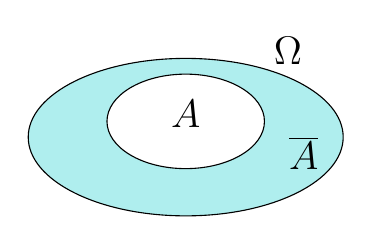
\begin{tikzpicture}
    \begin{scope}   [rotate=-90]
%     \draw [pattern color=blue, pattern=north east lines]  (0,0)  circle  (1 and 2);
    \fill [color=PaleTurquoise]  (0,0)  circle  (1 and 2);    
    \fill [color=white]  (0,0) ++(0:-.2) circle (.6 and 1);
    \draw (0,0)  circle  (1 and 2); 
    \draw (0,0) ++(0:-.2) circle (.6 and 1); 
    \end{scope} 
    \draw (1.5,-0.2) node {\Large $\overline{A}$ } ; 
    \draw (0,.3) node {\Large $A$} ; 
    \draw (1.3,1.1) node {\Large $\Omega$} ; 
    \end{tikzpicture} \\
    &       \\                
\end{tabular} 
\end{center}

% ------------------- Dessin A inter B -----------

\begin{center}
\begin{tabular}{c@{$\qquad \qquad$}c}
\raisebox{15ex}{\parbox{9cm}{
\textbf{2.} $ A \cap B $ est l'événement intersection de A et de B. \\ $x\in A\cap B \Longleftrightarrow x \in A \;  \mathbf{et} \; x \in B $.  \\ }}
  & \def\A_rond{(0,0)  circle  (1 and 2)}
\def\B_rond{(1,1)  circle  (1 and 2)}
\def\GrandRond{(2:0) circle (2.5 and 4)}

% On trace les ensembles 
\begin{tikzpicture}[scale=.6]

% On materialise l'intersection      
    \begin{scope}  [rotate=-30]
      \clip \A_rond;
      \clip \B_rond;
      \fill[color=PaleTurquoise] \GrandRond;
    \end{scope}
% On trace les bords ensuite       
    \begin{scope}  [rotate=-30]
    \draw \A_rond node[left] {$A$};
    \draw \B_rond node [right] {$B$};
    \draw \GrandRond node [above=2] {$\Omega$};
     \end{scope}     
\end{tikzpicture}\\
    &       \\                      
\end{tabular} 
\end{center}


\begin{center}
\begin{tabular}{c@{$\qquad \qquad$}c}
\raisebox{15ex}{\parbox{9cm}{
\textbf{3.} $ A \cup B $ est l'événement réunion de A et de B. \\ $ x \in A \cup B \Longleftrightarrow x \in A \; \mathbf{ou} \;  x \in B$.}}
  & \def\A_rond{(0,0)  circle  (1 and 2)}
\def\B_rond{(1,1)  circle  (1 and 2)}
\def\GrandRond{(2:0) circle (2.5 and 4)}

% On trace les ensembles 
\begin{tikzpicture}[scale=.6]
% On materialise l'union      
    \begin{scope}  [rotate=30]
      \clip \GrandRond ;
      \fill[color=PaleTurquoise] \A_rond \B_rond ; % ;
    \end{scope}
% On trace les bords ensuite     
    \begin{scope}  [rotate=30]
    \draw \A_rond node[left] {$A$};
    \draw \B_rond node [right] {$B$};
    \draw \GrandRond node [above=2.1] {$\Omega$};
     \end{scope} 
\end{tikzpicture}\\
    &       \\                      
\end{tabular} 
\end{center}

\newpage 

\section{Lois de De Morgan}

On jette un dé non pipé. \\

Univers $\Omega = \lb 1\; ; \; 2 \; ; \; 3 \; ; \; 4 \; ; \; 5 \; ; \; 6 \rb $.

Événement A : « Le résultat est pair » $ A = \lb 2 \; ; \; 4 \; ; \; 6 \rb $. \\

Événement B : « Le résultat est supérieur ou égal à 3 » $ B = \lb 3\; ; \; 4 \; ; \; 5 \; ; \; 6 \rb $ \\

On a : 

\begin{itemize}
\item[*] $ \overline{A} = \lb 1\; ; \; 3 \; ; \; 5\rb $ \\
\item[*] $ \overline{B} = \lb 1 \; ; \; 2 \rb $ \\
\item[*] $ A \cap B = \lb 4 \; ; \; 6 \rb $ \\
\item[*] $ A \cup B = \lb 2 \; ; \; 3 \; ; \; 4 \; ; \; 5 \; ; \; 6 \rb $ \\
\item[*] $ \overline{A \cap B} = \lb 1 \; ; \; 2 \; ; \;  3 \; ; \; 5 \rb $ \\
\item[*] $\overline{A \cup B} = \lb 1 \rb $ \\
\item[*] $ \overline{A} \cap \overline{B} = \lb 1 \rb $ \\
\item[*] $ \overline{A} \cup \overline{B} = \lb 1 \; ; \; 2 \; ; \; 3 \; ; \; 5 \rb $ \\
\end{itemize}

On constate que : 

\begin{itemize}
\item[*] $ \overline{A} \cap \overline{B} = \overline{A \cup B} $ \\
\item[*] $ \overline{A} \cup \overline{B} = \overline{A \cap B} $ \\
\end{itemize}


\tikzstyle{reverseclip}=[insert path={(current page.north east) --
  (current page.south east) --
  (current page.south west) --
  (current page.north west) --
  (current page.north east)}
]

\def\A_rond{(0,-.5)  circle  (1 and 2.5)}
\def\B_rond{(1,1)  circle  (1 and 2)}
\def\GrandRond{(2:0) circle (3.5 and 4)}

\begin{center}
\begin{tabular}{cc}

\begin{tikzpicture}[remember picture, scale=.4]

%------- Non (A inter B) 

\begin{scope}  [rotate=90]
    \fill [PaleTurquoise] \GrandRond;
\end{scope}

\begin{scope}  [rotate=90]
    \clip \A_rond;
    \clip \B_rond;
    \fill [color=white] \GrandRond;    
    \draw [color=white, pattern=north east lines] \GrandRond;
\end{scope}

\begin{scope}  [rotate=90]
    \draw \A_rond node[below] {$A$};
    \draw \B_rond node [above] {$B$};    
    \draw \GrandRond node [right=1.8cm ] {\Large $\overline{A \cap B}$};
\end{scope}
\end{tikzpicture} & 
\begin{tikzpicture}[remember picture, scale=.4] 

%------- (Non A) union (non B) ------------

% Je verdis non A 
\begin{scope}  [rotate=90]
   \begin{pgfinterruptboundingbox}
        \path  [clip] \A_rond  [reverseclip];
    \end{pgfinterruptboundingbox}
     \draw [opacity=0.5, pattern color=PaleGreen!60, 
           pattern=north east lines] \GrandRond;
\end{scope}

\begin{scope}  [rotate=90]    
   \begin{pgfinterruptboundingbox}
       \path  [clip] \B_rond [reverseclip];     
    \end{pgfinterruptboundingbox}
    \fill [opacity=0.5, pattern color=Salmon!60,
           pattern=fivepointed stars] \GrandRond;   
\end{scope}

\begin{scope}  [rotate=90]
    \clip \A_rond;
    \clip \B_rond;  
    \draw [pattern=north east lines] \GrandRond;    
\end{scope}

 \begin{scope}  [rotate=90]
    \draw \A_rond node[below] {$A$};
    \draw \B_rond node [above] {$B$};    
    \draw \GrandRond node [right=1.8cm ] 
            {\Large $\overline{A} \cup \overline{B}$};
\end{scope}
\end{tikzpicture} \\
 & \begin{tikzpicture} 
    \draw [opacity=0.5, pattern color=PaleGreen!60, 
           pattern=north east lines]
          (-3,0)   rectangle  (-1,.5) ;
         \draw (-2,.5)  node [above] {\Large $\overline{A}$}   ; 
        \draw [opacity=0.5, pattern color=Salmon!60,
           pattern=fivepointed stars]
          (0,0)  rectangle   (2,.5) ;      
         \draw (1,.5)  node [above] {\Large $\overline{B}$}   ; 
    \end{tikzpicture} \\
    & \\
%------- non (A union B )
\begin{tikzpicture}[remember picture, scale=.4] 
\begin{scope}  [rotate=90]
    \begin{pgfinterruptboundingbox}
        \path  [clip] \A_rond [reverseclip];
        \path  [clip] \B_rond [reverseclip];
    \end{pgfinterruptboundingbox}
     \fill [PaleTurquoise] \GrandRond;
\end{scope}

\begin{scope}  [rotate=90]
    \fill [pattern=north east lines] \A_rond  \B_rond;
\end{scope}

\begin{scope}  [rotate=90]
    \draw \A_rond node[below] {$A$};
    \draw \B_rond node [above] {$B$};    
    \draw \GrandRond node [right=1.8cm ]  {\Large $\overline{A \cup B}$};
\end{scope}
\end{tikzpicture} & 
\begin{tikzpicture}[remember picture, scale=.4] 

%-------  (non A) inter (non B)  
\begin{scope}  [rotate=90]
   \begin{pgfinterruptboundingbox}
        \path  [clip] \A_rond  [reverseclip];
    \end{pgfinterruptboundingbox}
     \draw [opacity=0.5, pattern color=PaleGreen!60, 
           pattern=north east lines] \GrandRond;
\end{scope}

\begin{scope}  [rotate=90]    
   \begin{pgfinterruptboundingbox}
       \path  [clip] \B_rond [reverseclip];     
    \end{pgfinterruptboundingbox}
    \fill [opacity=0.5, pattern color=Salmon!60,
           pattern=fivepointed stars] \GrandRond;   
\end{scope}

\begin{scope}  [rotate=90] 
    \fill [white] \A_rond \B_rond ;    
    \fill [pattern=north east lines] \A_rond \B_rond ;    
\end{scope}

 \begin{scope}  [rotate=90]
    \draw \A_rond node[below] {$A$};
    \draw \B_rond node [above] {$B$};    
    \draw \GrandRond node [right=1.8cm ] {\Large $\overline{A} \cap \overline{B}$};
\end{scope}
\end{tikzpicture} \\
\end{tabular}
\end{center}

\newpage

\section{Probabilité et espace probabilisé fini}

\subsection{Définition}

Soit $\Omega$ un univers.

On appelle \underline{probabilité} sur $\Omega$ toute fonction $p$ : $\mathcal{P}\left (\Omega\right ) \longrightarrow \R $

$\;  \;  \;  \;  \;  \;  \;  \;  \;  \; \;  \;  \;  \;  \; \; \; \;   \;  \;  \;  \; \;  \;  \;  \;  \;  \;  \;  \;  \;  \; \;  \;  \;  \;  \;  \;  \;  \;  \;  \;  \;  \;  \;  \;  \;  \;  \;  \;  \;  \; \;  \;  \;  \;  \;  \;  \;  \;  \;  \; \;  \;  \;  \;  \;  \;  \;  \;  \;  \;  \;  \;  \; \;  \;  \;  \;  \;  \;  \;  \;  \;  \; \;  \;  \;  \;  \;  \;  \;  \;  \;  \; \;  \;  \;  \;  \;  \;  \;  \;  \;  \; \;  \;  \;  \;  \;  \;  \;  \;  \;  \; \;  \;  \;  \;  \;  \;  \;  \; A  \;  \; \longmapsto p\left (A\right )$ \\

telle que : \\

\textbf{Premier axiome :} La probabilité de l'événement certain est égale à 1 : $p\left(\Omega\right) = 1$. \\

\textbf{Deuxième axiome : } Pour tout $A \in \mathcal{P}\left (\Omega\right )$, on a $ p\left(A\right) \geqslant 0$. \\

\textbf{Troisième axiome :} Pour tout $A \in \mathcal{P}\left (\Omega\right )$ et pour tout $B \in \mathcal{P}\left (\Omega\right )$,  \\ si $A \cap B = \varnothing$, c'est-à-dire si A et B sont incompatibles, alors $p\left(A\cup B\right) = p \left(A\right) + \left(B \right)$.

\subsection{Théorèmes fondamentaux}

Soit $\Omega$ un univers. Soit $p$ une probabilité définie sur $\Omega$. \\

\begin{itemize}
\item[*] Pour tout $A \in \mathcal{P}\left (\Omega\right )$, on a $p\left(\overline{A}\right) = 1 - p\left(A\right)$. \\ En particulier, $p\left(\varnothing\right) = p\left(\overline{\Omega}\right) = 1 - p\left(\Omega\right) = 1 - 1 = 0$. \\ La probabilité de l'événement impossible est donc nulle. \\

\item[*] Pour tout $A \in \mathcal{P}\left (\Omega\right )$ et pour tout $B\in \mathcal{P}\left (\Omega\right )$ : \\ Si $A \subset B$, alors $p\left(A\right) \leqslant p\left(B\right)$. \\ Ainsi, pour tout $A \in \mathcal{P}\left (\Omega\right )$, on a : $0 \leqslant p\left(A\right) \leqslant 1$. \\

\item[*] Pour tout $A\in \mathcal{P}\left (\Omega\right )$ et pour tout $B \in \mathcal{P}\left (\Omega\right )$, on a : $p\left(A\cup B\right) = p\left(A\right) + p\left(B\right) - p\left(A\cap B\right).$ \\
\end{itemize}

\subsection{Récapitulation}

\begin{itemize}
\item[*]$0 \leqslant p\left(A\right) \leqslant 1$. \\
\item[*] $p\left( \varnothing\right) = 0 $ et $ p\left(\Omega\right) = 1$ \\
\item[*] $p\left(\overline{A}\right) = 1 - p\left(A\right) $ \\
\item[*] $p\left( A \cup B \right) = p \left(A \right) - p \left(B \right) - p\left(A \cap B\right) $. \\
\end{itemize}

\vspace*{.3cm}

Enfin, on appelle \underline{espace probabilisé fini} tout univers dans lequel on a défini une probabilité.

\newpage

\section{Espace probabilisé fini dans lequel les événements sont équiprobables}

Soit $\Omega$ un univers tel que $\mathrm{card} \; \Omega = n$. \\
 
$\Omega = \lb \omega_1 \; ; \; \omega_2 \; ; \; \omega_3 \; ; \;  ... \; ; \; \omega_n \rb $ \\
 
On suppose que $p\left( \lb \omega_1 \rb \right) = p\left( \lb \omega_2 \rb \right) = p\left( \lb \omega_3 \rb \right) = ... = p\left( \lb \omega_n \rb \right) = p_0 $. \\
 
On a aussi : $\Omega = \lb \omega_1 \rb \cup \lb \omega_2 \rb \cup \lb \omega_3 \rb \cup ... \cup \lb \omega_n \rb = \displaystyle\bigcup_{i=1}^n \; \omega_i$ \\
 
Les événements élémentaires distincts sont incompatibles. \\ D'où : $p\left(\Omega\right) = p\left(\omega_1\right) + p\left(\omega_2\right) + p\left(\omega_3\right) + ... + p\left(\omega_n\right)$. \\

$p\left(\Omega\right) = p_0 + p_0 + p_0 + ... + p_0 $ \\

$p\left(\Omega\right) = np_0$ \\

Or, on sait que : $p\left(\Omega\right) = 1$. \\

Donc $np_0 = 1 $ \\

et $ p_0 = \dfrac{1}{n} $. \\

Soit A un événement quelconque non impossible, tel que $\mathrm{card} \; A = k$ avec $k \leqslant n$. \\

$A = \lb \omega_1 \; ; \;  \omega_2 \; ; \; \omega_3 \; ; \; ... \; ; \; \omega_k \rb $ \\

$p\left(A\right) = kp_0$ \\

$ p\left(A\right) = \dfrac{k}{n} $ \\

Soit $\Omega$ un univers dans lequel les événements élémentaires sont équiprobables. \\ Soit $A$ un événement quelconque tel que $\mathrm{card} \;  A = k$  \\

$ p\left(A\right) = \dfrac{\mathrm{card} \; A}{\mathrm{card} \; \Omega} $ \\

Et si $ A = \varnothing $ ? \\ 

$ p \left(A\right) = p \left(\varnothing\right) = 0 $ \\

$\dfrac{\mathrm{card} \; A}{\mathrm{card} \; \Omega} = \dfrac{\mathrm{card} \; \varnothing }{\mathrm{card} \; \Omega} = \dfrac{0}{n} = 0 $ \\

\newpage

\section{Exemples}

\subsection{Exemple \no 1}

Soit un jeu de 52 cartes. On tire une carte.

Événement A : « On tire un pique. » \\
Événement B : « On tire une carte rouge. » \\
Événement C : « On tire une figure. » \\

$\Omega =$ ensemble des 52 cartes du jeu. Donc $\mathrm{card} \; \Omega = 52$. 

\begin{itemize}
\item[*] $A = $ ensemble des piques, et $\mathrm{card} \; A = 13$ \\ $p\left(A\right) = \dfrac{\mathrm{card} \; A}{\mathrm{card} \; \Omega} = \dfrac{13}{52} = \dfrac{1}{4} $ \\
\item[*] $B = $ ensemble des cartes rouges, et $\mathrm{card} \; B = 26$ \\ $p\left(B\right) = \dfrac{\mathrm{card} \; B}{\mathrm{card} \; \Omega} = \dfrac{26}{52} = \dfrac{1}{2} $ \\
\item[*] $C = $ ensemble des figures, et $\mathrm{card} \; C = 12$ \\ $p\left(C\right) = \dfrac{\mathrm{card} \; C}{\mathrm{card} \; \Omega} = \dfrac{12}{52} = \dfrac{3}{13} $ \\
\item[*] $A\cap B = $ ensemble des piques rouges, et $\mathrm{card} \; \left(A \cap B\right) = 0$ \\ $p\left(A \cap B\right) = 0$ car A et B sont incompatibles. \\
\item[*] $A \cap C = $ ensemble des figures piques, et $\mathrm{card} \; \left(A \cap C\right) = 3$ \\ $p\left(A \cap C \right) = \dfrac{ \mathrm{card} \; \left(A \cap C\right)}{\mathrm{card} \; \Omega} = \dfrac{3}{52} $ \\
\item[*] $A \cup B = $ ensemble des piques ou des cartes rouges \\ $p\left(A \cup B\right) = p\left(A\right) + p\left(B\right)$ car A et B sont incompatibles. \\ $p\left(A \cup B\right) = \dfrac{1}{4} + \dfrac{1}{2} = \dfrac{3}{4} $ \\
\item[*]  $ A \cup C =$ ensembles des piques ou des figures ou les deux. \\ $p\left(A \cup C\right) = p\left(A\right) + p\left(C\right) - p\left(A \cap C\right) $ \\ $p\left(A \cup C\right) = \dfrac{1}{4} + \dfrac{3}{13} - \dfrac{3}{52} = \dfrac{11}{26} $ \\
\end{itemize}

Soit un événement E : « On tire ni un pique ni une carte rouge. » \\  Ainsi, la probabilité de tirer un trèfle est $p\left(E\right) = \dfrac{1}{4} $.

Autre méthode : $E = \overline{A} \cap \overline{B} = \overline{A \cup B}$. 

$p\left(E\right) = p\left(\overline{A\cup B}\right) = 1 - p\left(A \cup B\right) $

$p\left(E\right) = 1 - \dfrac{3}{4} $ 

$p\left(E\right) = \dfrac{1}{4} $ \\

Soit un événement F : « On tire ni un pique ni une figure. »

$F = \overline{A} \cap \overline{C} = \overline{A \cup C}$. 

$p\left(F\right) = p\left(\overline{A\cup C}\right) = 1 - p\left(A \cup C\right) $ 

$p\left(F\right) = 1 - \dfrac{11}{26} $ 

$p\left(F\right) = \dfrac{15}{26} $ 

\newpage

\subsection{Exercice \no 2}

\textbf{Première partie} \\

On jette un dé non pipé. \\ 

Soit un événement A : « Le résultat est pair. » \\

$\Omega = \lb 1,2,3,4,5,6 \rb $, avec $\mathrm{card} \; \Omega = 6$. \\

$ A = \lb 2,4,6 \rb $ et $ \mathrm{card} \; A = 3$. \\

$p\left(A\right) = \dfrac{\mathrm{card} \; A}{\mathrm{card} \; \Omega} = \dfrac{3}{6} = \dfrac{1}{2} $ \\

\textbf{Deuxième partie} \\

On jette 2 dés non pipés. \\ 

Soit un événement B : « La sommes des résultats est supérieure ou égale à 10. » \\

$\Omega = \lb 1,2,3,4,5,6 \rb \times \lb 1,2,3,4,5,6 \rb$, avec $\mathrm{card} \; \Omega = 6 \times 6 = 36$. \\

$B = \lb \left(4,6\right) \left(5,6\right) \left(5,5\right) \left(5,6\right) \left(6,5\right) \left(6,4\right) \rb $, avec $\mathrm{card} \; B = 6 $ \\

$p\left(B\right) = \dfrac{\mathrm{card} \; B}{\mathrm{card} \; \Omega} = \dfrac{6}{36} = \dfrac{1}{6} $ \\

\textbf{Troisième partie} \\

On jette 3 dés non pipés. \\ Soit un événement C : « On fait 421. » \\

$\Omega = \lb 1,2,3,4,5,6 \rb \times \lb 1,2,3,4,5,6 \rb \times \lb 1,2,3,4,5,6 \rb$ , avec $\mathrm{card} \; \Omega = 6 \times 6 \times 6 = 216$. \\

$C = \lb \left(4,2,1\right) \left(4,1,2\right) \left(2,4,1\right) \left(2,1,4\right) \left(1,4,2\right) \left(1,2,4\right) \rb $, avec $\mathrm{card} \; C = 6 $ \\

$p\left(C\right) = \dfrac{\mathrm{card} \; C}{\mathrm{card} \; \Omega} = \dfrac{6}{216} = \dfrac{1}{36} $ \\

\newpage

\subsection{Amusette \no 1}

On jette deux dés non pipés. On s'intéresse à la sommes des résultats, et on appelle $A$ cette somme. \\ Quelle est l'événement qui a la probabilité la plus élevée ? \\

\begin{itemize}
\item[*] $p\left(A = 1\right) = 0 $ \\
\item[*] $p\left(A = 2\right) = \dfrac{1}{36} $ \\
\item[*] $p\left(A = 3\right) = \dfrac{1}{18} $ \\
\item[*] $p\left(A = 4\right) = \dfrac{1}{12} $ \\
\item[*] $p\left(A = 5\right) = \dfrac{1}{9} $ \\
\item[*] $p\left(A = 6\right) = \dfrac{5}{36} $ \\
\item[*] $p\left(A = 7\right) = \dfrac{1}{6} $ \\
\item[*] $p\left(A = 8\right) = \dfrac{5}{36} $ \\
\item[*] $p\left(A = 9\right) = \dfrac{1}{9} $ \\
\item[*] $p\left(A = 10\right) = \dfrac{1}{12} $ \\
\item[*] $p\left(A = 11\right) = \dfrac{1}{18} $ \\
\item[*] $p\left(A = 12\right) = \dfrac{1}{36}  $ \\
\end{itemize}

L'événement $A=7$ a donc la probabilité la plus élevée. \\

\textbf{Remarque :} La somme des probabilités est bien égale à 1.

\newpage

\subsection{Amusette \no 2}

On jette un dé pipé. \\Les nombres 1,2,3,4, et 5 ont la même probabilité de sortie, mais la probabilité d'obtenir un 6 est égale \\ à 3 fois la probabilité d'obtenir un 1. \\

Déterminer la probabilité de sortie de chaque nombre. \\

$p\left(X=1\right) = p\left(X=2\right) = p\left(X=3\right) = p\left(X=4\right) = p\left(X=5\right) = p_0 $ \\

$p\left(X=6\right) = 3p\left(X=1\right) = 3p_0 $ \\

On a $p\left(X=1\right) + p\left(X=2\right) + p\left(X=3\right) + p\left(X=4\right) + p\left(X=5\right) + p\left(X=6\right) = 1$ \\

$ p_0 + p_0 + p_0 + p_0 + p_0 + 3p_0 = 1 $ \\

$ 5p_0 + 3p_0 = 1 $ \\

$ 8p_0 = 1 $ \\

 $p_0 = \dfrac{1}{8} $ \\
 
Donc :

\begin{itemize}
\item[*] $p\left(X=1\right) = \dfrac{1}{8} $ \\
\item[*] $p\left(X=2\right) = \dfrac{1}{8} $ \\
\item[*] $p\left(X=3\right) = \dfrac{1}{8} $ \\
\item[*] $p\left(X=4\right) = \dfrac{1}{8} $ \\
\item[*] $p\left(X=5\right) = \dfrac{1}{8} $ \\
\item[*] $p\left(X=6\right) = \dfrac{3}{8} $ \\
\end{itemize}

\newpage

\subsection{Exercice \no 3}

Soit une urne contenant deux boules rouges et trois boules blanches. \\

\textbf{Première partie} \\

Soit un événement A : « On tire une boule rouge. » \\

Quelle est la probabilité de A ? \\

$ \Omega = \lb R_1, R_2, B_1, B_2, B_3 \rb $, et $\mathrm{card} \; \Omega = 5 $ \\

$ A = \lb R_1, R_2 \rb $, et $ \mathrm{card} \; A = 2 $ \\

$ p\left(A\right) = \dfrac{\mathrm{card} \; A}{\mathrm{card} \; \Omega} = \dfrac{2}{5} $ \\

\textbf{Deuxième partie} \\

On tire deux boules simultanément. \\ Soit un événement A : « On tire deux boules rouges. » \\Soit un événement B : « On tire une boule rouge et une boules blanche. » \\Soit un événement C : « On tire deux boules blanches. » \\

$\Omega = \lb \lb R_1,R_2 \rb \lb R_1,B_1 \rb \lb R_1,B_2 \rb \lb R_1,B_3 \rb \lb R_2,B_1 \rb \lb R_2,B_2 \rb \lb R_2,B_3 \rb \lb B_1,B_2 \rb \lb B_1,B_3 \rb \lb B_2,B_3 \rb \rb  $, $\mathrm{card} \; \Omega = 10 $. \\

\textbf{Remarque :} $\Omega$ est un ensemble de paires de boules. \\

$A = \lb \lb R_1, R_2 \rb \rb $, et $\mathrm{card} \; A = 1 $ \\

$ p\left(A\right) = \dfrac{\mathrm{card} \; A}{\mathrm{card} \; \Omega} = \dfrac{1}{10}$ \\

\vspace*{.3cm}

$B = \lb \lb R_1, B_1 \rb \lb R_1, B_2 \rb\lb R_1, B_3 \rb\lb R_2, B_1 \rb \lb R_2, B_2 \rb \lb R_2, B_3 \rb \rb $, et $\mathrm{card} \; B = 6 $ \\

$ p\left(A\right) = \dfrac{\mathrm{card} \; B}{\mathrm{card} \; \Omega} = \dfrac{6}{10} = \dfrac{3}{5}$ \\

\vspace*{.3cm}

$B = \lb  \lb B_1, B_2 \rb \lb B_1, B_3 \rb \lb B_2, B_3 \rb \rb $, et $\mathrm{card} \; C = 3 $ \\

$ p\left(A\right) = \dfrac{\mathrm{card} \; C}{\mathrm{card} \; \Omega} = \dfrac{3}{10} $ \\

On vérifie que $p\left(A\right) + p\left(B\right) + p\left(C\right) = 1 $ \\

On a bien $\dfrac{1}{10} + \dfrac{6}{10} + \dfrac{3}{10} = 1 $

\newpage 

\subsection{Exercice \no 4}

Soit un jeu de 52 cartes. \\

\textbf{Première partie} \\

On tire successivement deux cartes avec remise. \\

$\Omega =$  ensemble des 52 cartes $ \times $ ensemble des 52 cartes, avec $\mathrm{card} \; \Omega = 52 \times 52 = 2704 $ \\

\begin{itemize}
\item[*] Soit un événement A : « On tire deux piques. » 
\item[*] Soit un événement B : « On ne tire pas de pique. » 
\item[*] Soit un événement C : « On tire au moins un pique. » 
\item[*] Soit un événement D : « On tire un pique et un seul. » 
\end{itemize}

\vspace*{.3cm }
$ A = $ ensemble des 13 piques $ \times $ ensemble des 13 piques, et $\mathrm{card} \; A = 13 \times 13 = 169 $ \\

$ p\left(A\right) = \dfrac{\mathrm{card} \; A}{\mathrm{card} \; \Omega} = \dfrac{169}{2704} = \dfrac{1}{16} $ \\

$ B = $ \hbox{ensemble des 39 cartes non-piques $ \times $ ensemble des 39 cartes non-piques, et $\mathrm{card} \; B = 39 \times 39 = 1521 $.} \\

$ p\left(B\right) = \dfrac{\mathrm{card} \; B}{\mathrm{card} \; \Omega} = \dfrac{1521}{2704} = \dfrac{9}{16} $ \\

$ C = \overline{B} $ \\

$ p\left(C\right) = p\left(\overline{B} \right) = 1 - p\left(B\right) = 1 - \dfrac{9}{16} = \dfrac{7}{16} $ \\

$ D = \overline{A} \cap \overline{B} = \overline{A \cup B} $ \\

$ p\left(D\right) = p\left(\overline{A\cup B}\right) = 1 - p\left(A\cup B\right)$.  \\

Or, $p\left(A\cup B\right) = p\left(A\right) + p\left(B\right) $ car A et B sont incompatibles. \\

Ainsi $p\left(A\cup B\right) = \dfrac{1}{16} + \dfrac{9}{16} = \dfrac{10}{16} = \dfrac{5}{8} $ \\

Et $p\left(D\right) = 1 - \dfrac{5}{8} = \dfrac{3}{8} $ \\

On vérifie que $\left(A\right) + \left(D\right) + \left(B\right) = 1$ (ensemble des cas possibles). \\ On constate d'ailleurs que $p\left(A\right) + p\left(B\right) + p\left(C\right) + p\left(D\right) \neq 1 $.

\newpage

\textbf{Seconde partie} \\

On tire successivement deux cartes sans remise. \\

$\Omega =$  ensemble des 52 cartes $ \times $ ensemble des 51 cartes restantes, avec $\mathrm{card} \; \Omega = 52 \times 51 = 2652 $. \\

$ A = $ ensemble des 13 piques $ \times $ ensemble des 12 piques restants, et $\mathrm{card} \; A = 13 \times 12 = 156 $ \\

$ p\left(A\right) = \dfrac{\mathrm{card} \; A}{\mathrm{card} \; \Omega} = \dfrac{156}{2652} = \dfrac{1}{17} $ \\

$ B = $ ensemble des 39 cartes non-piques $ \times $ ensemble des 38 cartes non-piques restantes, et $\mathrm{card} \; B = 39 \times 38 = 1482 $ \\

$ p\left(B\right) = \dfrac{\mathrm{card} \; B}{\mathrm{card} \; \Omega} = \dfrac{1482}{2652} = \dfrac{19}{34} $ \\

$ C = \overline{B} $ \\

$ p\left(C\right) = p\left(\overline{B} \right) = 1 - p\left(B\right) = 1 - \dfrac{19}{34} = \dfrac{15}{34} $ \\

$ D = \overline{A} \cap \overline{B} = \overline{A \cup B} $ \\

$ p\left(D\right) = p\left(\overline{A\cup B}\right) = 1 - p\left(A\cup B\right)$.  \\

Or, $p\left(A\cup B\right) = p\left(A\right) + p\left(B\right) $ car A et B sont incompatibles. \\

Ainsi $p\left(A\cup B\right) = \dfrac{1}{17} + \dfrac{19}{34} = \dfrac{21}{34} $ \\

Et $p\left(D\right) = 1 - \dfrac{21}{34} = \dfrac{13}{34} $ \\

On vérifie que $p\left(A\right) + p\left(D\right) + p\left(B\right) = 1$ (ensemble des cas possibles). On constate d'ailleurs que $p\left(A\right) + p\left(B\right) + p\left(C\right) + p\left(D\right) \neq 1 $.

\newpage

\section{Événements indépendants : Exercice, le Pachinko}

Soit $\Omega$ un univers. \\ Soit $p$ une probabilité définie sur $\Omega$. \\ Soient A et B deux événements sur $\Omega$. \\

A et B sont indépendants $ \Longleftrightarrow p\left(A \cap B \right) = p\left(A\right) \times p\left(B\right) $ \\

\textbf{Attention :} ne pas confondre « indépendants » et « incompatibles ». \\

\textbf{Schéma du Pachinko :}

\begin{center}

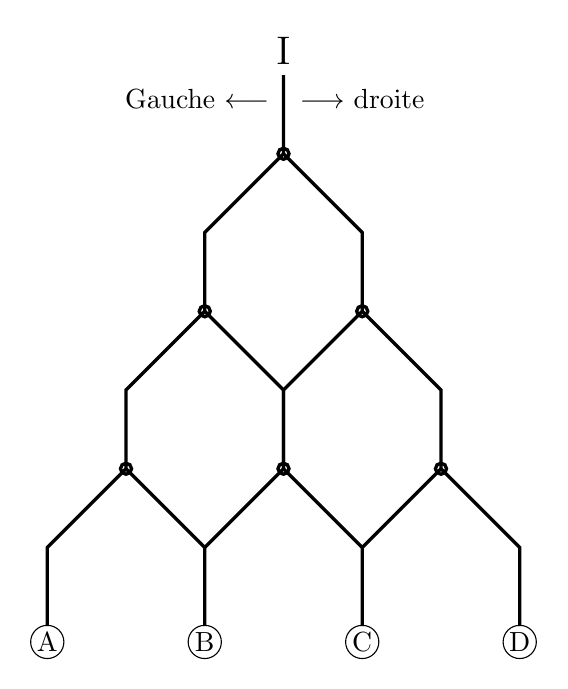
\begin{tikzpicture}[node distance=1cm]
% \draw[help lines, gray] (0,0) grid (7,8);
\draw (0,-.2) circle (6pt) ; \draw (0,-.2) node {A} ;
\draw (2,-.2) circle (6pt) ; \draw (2,-.2) node {B} ;
\draw (4,-.2) circle (6pt) ; \draw (4,-.2) node {C} ;
\draw (6,-.2) circle (6pt) ; \draw (6,-.2) node {D} ;
 \draw [very thick] (0,0) -- (0,1)   -- (1,2) circle (2pt)  -- (1,3) -- (2,4) circle (2pt)   -- (2,5) -- (3,6) circle (2pt)  -- (3,7) node (I) [above] {\Large I} ; 
\draw [very thick] (2,0) -- (2,1)   -- (1,2) ; 
\draw [very thick] (2,1) -- (3,2) circle (2pt)  -- (3,3) -- (2,4) ; 
\draw [very thick] (4,0) -- (4,1) -- (3,2) -- (3,3) -- (4,4) circle (2pt)  -- (4,5) -- (3,6) ;  
\draw [very thick] (4,1) -- (5,2)circle (2pt)   ; 
\draw [very thick] (6,0) -- (6,1) -- (5,2) -- (5,3) -- (4,4)  ; 
\draw ((2,6.7) node {Gauche $\longleftarrow \;\;$} ; 
\draw ((4,6.7) node {$\longrightarrow$ droite} ; 
\end{tikzpicture}

\end{center}

La probabilité qu'une boule lâchée en I prenne la direction « gauche » \\ à une intersection est de $\dfrac{1}{3} $. Les événements successifs sont indépendants. \\

Soit $G_i$ l'événement : « La boule prend la direction gauche à la $i^\mathrm{ème}$ intersection. »

$p\left(G_1\right) = p\left(G_2\right) = p\left(G_3\right) = p\left(G_4\right) = p\left(G_5\right) = p\left(G_6\right) = p\left(G\right) =  \dfrac{1}{3}$. \\

$p\left(\overline{G}\right) = 1 - p\left(G\right) = 1 - \dfrac{1}{3} = \dfrac{2}{3} $ \\

Soit un événement A : « La boule arrive en A. » \\

$ A = G \cap G \cap G $ \\

$ p\left(A\right) = p\left(G \cap G \cap G\right) = p\left(G\right) \times p\left(G\right) \times p\left(G\right) = \dfrac{1}{3} \times \dfrac{1}{3} \times \dfrac{1}{3} = \left(\dfrac{1}{3}\right)^3 = \dfrac{1}{27} $ \\

\newpage

Soit un événement B : « La boule arrive en B. » \\

$ B = \left( G \cap G \cap \overline{G} \right) \cup \left( G \cap \overline{G} \cap G \right) \cup \left( \overline{G} \cap G \cap G \right) $ \\

Ces trois éléments sont incompatibles deux à deux. \\

$ p\left(B\right) = p\left[\left( G \cap G \cap \overline{G} \right) \cup \left( G \cap \overline{G} \cap G \right) \cup \left( \overline{G} \cap G \cap G \right)\right] $ \\

$ p\left(B\right) = p\left( G \cap G \cap \overline{G} \right) +  p\left( G \cap \overline{G} \cap G \right) +  p\left( \overline{G} \cap G \cap G \right) $ \\

$ p\left(B\right) = p\left(G\right) \times p\left(G\right) \times p\left(\overline{G}\right) + p\left(G\right) \times p\left(\overline{G}\right) \times p\left(G\right) + p\left(\overline{G}\right) \times p\left(G\right) \times p\left(G\right) $ \\

$ p\left(B\right) = \dfrac{1}{3} \times \dfrac{1}{3} \times \dfrac{2}{3} +  \dfrac{1}{3} \times \dfrac{2}{3} \times \dfrac{1}{3} +  \dfrac{2}{3} \times \dfrac{1}{3} \times \dfrac{1}{3} $ \\

$ p\left(B\right) = \left(\dfrac{1}{3}\right)^2 \times \dfrac{2}{3} +  \left(\dfrac{1}{3}\right)^2 \times \dfrac{2}{3} +  \left(\dfrac{1}{3}\right)^2 \times \dfrac{2}{3} $ \\

$ p\left(B\right) = 3\left(\dfrac{1}{3}\right)^2 \times \dfrac{2}{3} $ \\

$ p\left(B\right) = \dfrac{2}{9} $ \\

Soit un événement C : « La boule arrive en C. » \\

$ C = \left( \overline{G} \cap  \overline{G} \cap G \right) \cup \left( \overline{G} \cap G \cap \overline{G} \right) \cup \left( G \cap \overline{G} \cap \overline{G} \right) $ \\

Ces trois éléments sont incompatibles deux à deux. \\

$ p\left(C\right) = p\left[\left( \overline{G} \cap  \overline{G} \cap G \right) \cup \left( \overline{G} \cap G \cap \overline{G} \right) \cup \left( G \cap \overline{G} \cap \overline{G} \right)\right] $ \\

$ p\left(C\right) = p\left(\overline{G} \cap  \overline{G} \cap G \right) + p\left( \overline{G} \cap G \cap \overline{G} \right) + p\left( G \cap \overline{G} \cap \overline{G} \right) $ \\

$ p\left(C\right) = p\left(\overline{G}\right) \times p\left(\overline{G}\right) \times p\left(G\right) + p\left(\overline{G}\right) \times p\left(G\right) \times p\left(\overline{G}\right) + p\left(G\right) \times p\left(\overline{G}\right) \times p\left(\overline{G}\right) $ \\

$ p\left(C\right) = \dfrac{2}{3} \times \dfrac{2}{3} \times \dfrac{1}{3} +  \dfrac{2}{3} \times \dfrac{1}{3} \times \dfrac{2}{3} +  \dfrac{1}{3} \times \dfrac{2}{3} \times \dfrac{2}{3} $ \\

$ p\left(C\right) = \left(\dfrac{2}{3}\right)^2 \times \dfrac{1}{3} +  \left(\dfrac{2}{3}\right)^2 \times \dfrac{1}{3} +  \left(\dfrac{2}{3}\right)^2 \times \dfrac{1}{3} $ \\

$ p\left(C\right) = 3\left(\dfrac{2}{3}\right)^2 \times \dfrac{1}{3} $ \\

$ p\left(C\right) = \dfrac{4}{9} $ \\

Soit un événement D : « La boule arrive en D. » \\

$ D = \overline{G} \cap \overline{G} \cap \overline{G} $ \\

$ p\left(D\right) = p\left(\overline{G} \cap \overline{G} \cap \overline{G}\right) = p\left(\overline{G}\right) \times p\left(\overline{G}\right) \times p\left(\overline{G}\right) = \dfrac{2}{3} \times \dfrac{2}{3} \times \dfrac{2}{3} = \left(\dfrac{2}{3}\right)^3 = \dfrac{8}{27} $ \\

On vérifie que $p\left(A\right) + p\left(B\right) + p\left(C\right) + p\left(D\right) = 1$.

\newpage

\section{Variable aléatoire, loi de probabilité et espérance mathématique}

\subsection{Exemple}

On investit un euro. \\ On tire une carte dans un jeu de 52 cartes. On gagne 4 euros si la carte tirée est un cœur. On perd sa mise sinon. \\

\begin{itemize}
\item[•] Soit $X$ la \textbf{variable aléatoire} qui correspond au gain du jouer. \\ 

$X\left(\Omega\right) = \lb -1 \; ; \; 3 \rb$. \\
\item[•] \textbf{Loi de probabilité} de $X$ : \\
\end{itemize}

\begin{tabular}{|c|l|l|}
\hline
$x_i$ & $-1$ & $3$ \\
\hline
& & \\
$p\left(X = x_i\right)$ & $\dfrac{3}{4}$ & $\dfrac{1}{4}$ \\
& & \\
\hline
\end{tabular}

\vspace*{.3cm}

On a bien $p\left(X = -1\right) + p\left(X = 3\right) = 1$ \\

\begin{itemize}
\item[•] \textbf{Espérance mathématique} de X : \\
\end{itemize}

$E(x) = \displaystyle \sum  x_ip\left(X = x_i\right)$ \\

$ E(x) = -1 \times \dfrac{3}{4} + 3 \times \dfrac{1}{4} = 0$. \\

Donc le jeu est équilibré. \\

L'espérance mathématique s'apparente à la moyenne des gains, car on peut écrire : \\

$E(x) = \dfrac{3 \times \left(-1\right)+ 1 \times 3}{4}$, qui est de la forme : $\overline{x} = \dfrac{\Sigma n_ix_i}{\Sigma n_i}$ \\

\textbf{Remarque :} \\

\begin{itemize}
\item[*] Si $E(x) > 0$, alors le jeu est favorable au joueur.  
\item[*] Si $E(x) < 0$, alors le jeu est défavorable au joueur. 
\end{itemize} 

\newpage

\subsection{Sujet de bac}

Un fabricant d'objets périssables : \\

\begin{itemize}
\item[•] gagne $300$ euros par objet vendu.
\item[•] perd $200$ euros par objet invendu. 
\end{itemize}

\vspace*{.3cm}

On appelle $D$ la demande journalière. \\
On appelle $G_k$ la variable aléatoire correspondant au gain quotidien réalisé lorsque l'on fabrique $k$ objets avec $0 \leqslant k \leqslant 4$. \\

On donne : \\

\begin{tabular}{|c|c|c|c|c|c|c|}
\hline
& & & & & & \\
Demandes journalières $d_i$ & 0 & 1 & 2 & 3 & 4 & 5 ou plus \\
& & & & & & \\
\hline
& & & & & & \\
$p\left(D = d_i\right)$ & $0,1$ & $0,2$ & $0,35$ & $0,25$ & $0,1$ & $0$ \\
& & & & & & \\
\hline
& & & & & & \\
$G_1$ & $-200$ & $300$ & $300$ & $300$ & $300$ & $300$ \\
& & & & & & \\
\hline
& & & & & & \\
$G_2$ & $-400$ & $100$ & $600$ & $600$ & $600$ & $600$ \\
& & & & & & \\
\hline
& & & & & & \\
$G_3$ & $-600$ & $-100$ & $400$ & $900$ & $900$ & $900$ \\
& & & & & & \\
\hline
& & & & & & \\
$G_4$ & $-800$ & $-300$ & $200$ & $700$ & $1200$ & $1200$ \\
& & & & & & \\
\hline
\end{tabular}

\vspace*{.3cm}

On calcule l'espérance mathématique des différents gains : \\

$E(G_1) = -200 \times 0,1 + 300 \times 0,2 + 300 \times 0,35 + 300 \times 0,25 + 300 \times 0,1$ \\
$E(G_1) = 250$ \\

De même, on trouve : \\ 

$E(G_2) = 400$ \\

$E(G_3) = 375$ \\

$E(G_4) = 225$ \\

Donc l'artisan doit fabriquer $2$ objets pour espérer obtenir la gain le plus important. \\ La moyenne de ses gains sera alors de $400$ euros par jour.

\newpage

\vspace*{-2.3cm}

\section{Épreuves répétées}

On considère une expérience n'admettant que deux résultats possibles, appelés « succès » ou « échec~» et notés \\ respectivement $S$ et $\overline{S} $.

\vspace*{-.3cm}

\subsection{Épreuve de Bernoulli}

On répète l'épreuve dans des conditions identiques, les résultats successifs étant indépendants les uns des autres. 

\vspace*{-.3cm}

\subsection{Schéma de Bernoulli ou loi binomiale}

\textbf{Exemple}

On jette un dé non-pipé. \\ Soit un événement S : « On obtient un 6. » $p\left(S\right) = \dfrac{1}{6} $. \\

\underline{Épreuve de Bernoulli :} On jette le dé trois fois de suite. \\

\underline{Schéma de Bernoulli :} Soit \hbox{un événement A : « On obtient exactement deux fois 6 au cours des trois jets. »} \\

Quelle est la probabilité de A ? \\

\begin{tikzpicture} 
[level distance=10mm]
\tikzstyle{level 1}=[sibling distance=40mm]
\tikzstyle{level 2}=[sibling distance=20mm]
\tikzstyle{level 3}=[sibling distance=10mm]

\node (root) {}
[grow=right]
child {node {$\overline{S}$}
       child {node {$\overline{S}$}              
              child {node {$\overline{S}$}}
              child {node {$S$}} 
             }
       child {node {$S$}             
              child {node {$\overline{S}$}}
              child {node {$S$}} 
             }
      }
child {node {$S$}
       child {node {$\overline{S}$}
              child {node {$\overline{S}$}}
              child {node {$S$}} 
             }
       child {node {$S$}
              child {node {$\overline{S}$}}
              child {node {$S$}} 
             } 
      }
; 

\node at (root-2-2-2) [right] {$\qquad\qquad S\cap S\cap S \quad p(S)\times p(S) \times p(S) = \dfrac{1}{6} \times \dfrac{1}{6} \times \dfrac{1}{6} = \left(\dfrac{1}{6}\right)^3$} ; 
\node at (root-2-2-1) [right] {$\star \quad\qquad S\cap S\cap \overline{S} \quad p(S)\times p(S) \times p(\overline{S}) = \dfrac{1}{6} \times \dfrac{1}{6} \times \dfrac{5}{6} = \left(\dfrac{1}{6}\right)^2 \times \dfrac{5}{6}$} ; 
\node at (root-2-1-2) [right] {$\star \quad\qquad S\cap \overline{S}\cap S \quad p(S)\times p(\overline{S}) \times p(S) = \dfrac{1}{6} \times \dfrac{5}{6} \times \dfrac{1}{6} = \left(\dfrac{1}{6}\right)^2 \times \dfrac{5}{6}$} ; 
\node at (root-2-1-1) [right] {$\qquad\qquad S\cap \overline{S}\cap \overline{S} \quad p(S)\times p(\overline{S}) \times p(\overline{S}) = \dfrac{1}{6} \times \dfrac{5}{6} \times \dfrac{5}{6} = \dfrac{1}{6} \times \left(\dfrac{5}{6}\right)^2$} ; 
\node at (root-1-2-2) [right] {$\star \quad\qquad \overline{S}\cap S\cap S \quad p(\overline{S})\times p(S) \times p(S) = \dfrac{5}{6} \times \dfrac{1}{6} \times \dfrac{1}{6} = \left(\dfrac{1}{6}\right)^2 \times \dfrac{5}{6}$} ; 
\node at (root-1-2-1) [right] {$\qquad\qquad \overline{S}\cap S\cap \overline{S} \quad p(\overline{S})\times p(S) \times p(\overline{S}) = \dfrac{5}{6} \times \dfrac{1}{6} \times \dfrac{5}{6} = \dfrac{1}{6} \times \left(\dfrac{5}{6}\right)^2$} ; 
\node at (root-1-1-2) [right] {$\qquad\qquad \overline{S}\cap \overline{S}\cap S \quad p(\overline{S})\times p(\overline{S}) \times p(S) = \dfrac{5}{6} \times \dfrac{5}{6} \times \dfrac{1}{6} = \dfrac{1}{6} \times \left(\dfrac{5}{6}\right)^2$} ; 
\node at (root-1-1-1) [right] {$\qquad\qquad \overline{S}\cap \overline{S}\cap \overline{S} \quad p(\overline{S})\times p(\overline{S}) \times p(\overline{S}) = \dfrac{5}{6} \times \dfrac{5}{6} \times \dfrac{5}{6} = \left(\dfrac{5}{6}\right)^3$} ; 
\end{tikzpicture}

$ A = \left(S \cap S \cap \overline{S} \right) \cup \left(S \cap \overline{S} \cap S \right) \cup \left(\overline{S} \cap S \cap S\right)$. \\

Ces trois événements sont incompatibles deux à deux. \\

$ p\left(A\right) = p\left[\left(S \cap S \cap \overline{S} \right) \cup \left(S \cap \overline{S} \cap S \right) \cup \left(\overline{S} \cap S \cap S\right)\right] $ \\

$ p\left(A\right) = p\left(S \cap S \cap \overline{S} \right) + p\left(S \cap \overline{S} \cap S \right) + p\left(\overline{S} \cap S \cap S\right) $ \\

$ p\left(A\right) = \dfrac{1}{6} \times \dfrac{1}{6} \times \dfrac{5}{6} + \dfrac{1}{6} \times \dfrac{5}{6} \times \dfrac{1}{6} + \dfrac{5}{6} \times \dfrac{1}{6} \times \dfrac{1}{6} $ \\

$ p\left(A\right) =  \left(\dfrac{1}{6}\right)^2 \times \dfrac{5}{6} + \left(\dfrac{1}{6}\right)^2 \times \dfrac{5}{6} + \left(\dfrac{1}{6}\right)^2 \times \dfrac{5}{6} $ \\

$p\left(A\right) = 3 \left(\dfrac{1}{6} \right)^2 \times \dfrac{5}{6} $ \\

$ p\left(A\right) = \dfrac{5}{72} $

\vspace*{-5cm}

\newpage

\subsection{Généralisation}

Soit une épreuve de Bernoulli, avec $p$ la probabilité de succès de l'épreuve. \\
On répète l'épreuve $n$ fois dans des conditions identiques. \\ Les résultats étant indépendants les uns des autres. \\

\textbf{Schéma de Bernoulli de paramètres $\mathbf{n}$ et $\mathbf{p}$, ou loi binomiale :} $\mathbf{\mathcal{B} \left(n,p\right)}$ \\

Soit A l'événement « On obtient exactement k succès. » $p(A)$ est donnée par la formule : \\

$ p\left(A\right)  = \left(\begin{array}{c} n \\ k \end{array} \right) p^k \left(1-p\right)^{n-k} \; \;  $ avec $\left(\begin{array}{c} n \\ k \end{array} \right)$ le nombre de manières d'obtenir $k$ succès dans $n$ épreuves. \\

\textbf{Remarque :} On a $ 0 \leqslant k \leqslant n $.  \\

\textbf{Exemples :}

$\left(\begin{array}{c} 4 \\ 3 \end{array} \right)$ = 4. Il y a 4 façons d'obtenir trois succès quand l'épreuve est répétée quatre fois : \\

\begin{tabular}{l}
$ S \; S \; S \; \overline{S} $ \\
$ S \; S  \; \overline{S} \; S $ \\
$ S \; \overline{S} \; S \; S $ \\
$ \overline{S} \; S \; S \; S $ \\
\end{tabular}

\vspace{.3cm}

$\left(\begin{array}{c} 4 \\ 2 \end{array} \right)$ = 6. Il y a 6 façons d'obtenir deux succès quand l'épreuve est répétée quatre fois : \\

\begin{tabular}{l}
$ S \; S \; \overline{S} \; \overline{S} $ \\
$ S \; \overline{S} \; S \overline{S} $ \\
$ \overline{S} \; S \; S \overline{S} $ \\
$ S \; \overline{S}  \; \overline{S} \; S $ \\
$ \overline{S} \; S \; \overline{S} \; S $ \\
$ \overline{S} \; \overline{S} \; S \; S $ \\
\end{tabular}

\vspace{.3cm}

$\left(\begin{array}{c} 5 \\ 3 \end{array} \right)$ = 10. Il y a 10 façons d'obtenir trois succès quand l'épreuve est répétée cinq fois : \\

\begin{tabular}{l}
$ S \; S \; S\; \overline{S} \; \overline{S} $ \\
$ S \; S \overline{S} \; S \; \overline{S} $ \\
$ S \; \overline{S} \; S \; S \; \overline{S} $ \\
$ \overline{S}  \; S \; S \; S \overline{S} $ \\
$ S \; S \;  \overline{S} \; \overline{S} \; S $ \\
$ S \; \overline{S} \; S \; \overline{S} \; S $ \\
$ \overline{S} \; S \; S \; \overline{S} \; S $ \\
$ S \; \overline{S} \; \overline{S} \; S \; S $ \\
$  \overline{S} \; S \; \overline{S} \; S \; S $ \\
$  \overline{S} \; \overline{S} \; S \; S \; S $ \\
\end{tabular}

\vspace{.3cm}

\subsection{Triangle de Pascal}

%Papa + Texte à mettre en orange

\begin{tabular}{r@{$\;=\;$}lll}
\multicolumn{2}{l}{$\;\;\; a+b$} & $1 \;\;\; 1$ & $n=1$ \\
$(a+b)^2 $ & $ a^2 +2ab+b^2$ & $1 \;\;\; 2 \;\;\; 1 $ & $n =2$ \\
$(a+b)^3 $ & $ a^3 +3a^2b+3ab^2+b^3$ & $1 \;\;\; 3 \;\;\; 3 \;\;\;\; 1 $ & $n =3$ \\
$(a+b)^4 $ & $ a^4 + 4a^3b +6a^2 b^2 + 4ab^3 +b^4 $
           &  $1 \;\;\; 4 \;\;\; 6 \;\;\;\; 4 \;\;\;\; 1 $ & $n =4$ \\
$(a+b)^5 $ & $ a^5 + 5a^4b +10a^3 b^2 + 10a^2b^3 + 5ab^4 + b^5 $
           &  $1 \;\;\; 5 \; 10 \; 10 \;\;\;  5 \;\; 1 $ & $n =5$ \\    
$(a+b)^6 $ & $ a^6 + 6a^5b +15a^4 b^2 + 20a^3b^3 + 15a^2b^4 + 6ab^5 +b^6 $
           &  $1 \;\;\; 6 \; 15 \; 20 \; 15 \;  6 \;\;\; 1 $ & $n =6$ \\                     
\end{tabular}\\

\textcolor{orange} {\begin{tabular}{lccc}
Calculatrice : & 3 & combinaison & 2 \\
& 4 & combinaison & 2 \\
& 4 & combinaison & 3 \\
& 5 & combinaison & 3 \\
\end{tabular}}

\subsection{Loi de probabilité et espérance mathématique de la loi binomiale}

\textbf{Exemple :} $n = 3$ et $p = \dfrac{1}{6}$ \\

$p\left(X = 0\right) = \left(\begin{array}{c} 3 \\ 0 \end{array}\right) \left(\dfrac{1}{6}\right)^0\left(\dfrac{5}{6}\right)^3 = \left(\dfrac{5}{6}\right)^3 = \dfrac{125}{216}$ \vspace*{.3cm} \\

$p\left(X = 1\right) = \left(\begin{array}{c} 3 \\ 1 \end{array}\right) \left(\dfrac{1}{6}\right)^1\left(\dfrac{5}{6}\right)^2 = 3 \times \dfrac{1}{6} \left(\dfrac{5}{6}\right)^2 = \dfrac{25}{72}$ \vspace*{.3cm} \\

$p\left(X = 2\right) = \left(\begin{array}{c} 3 \\ 2 \end{array}\right) \left(\dfrac{1}{6}\right)^2\left(\dfrac{5}{6}\right)^1 = 3 \times \left(\dfrac{1}{6}\right)^2 \dfrac{5}{6} = \dfrac{5}{72}$ \vspace*{.3cm} \\

$p\left(X = 3\right) = \left(\begin{array}{c} 3 \\ 3 \end{array}\right) \left(\dfrac{1}{6}\right)^3\left(\dfrac{5}{6}\right)^0 = \left(\dfrac{1}{6}\right)^3 = \dfrac{1}{216}$ \vspace*{.3cm} \\

On vérifie que l'ensemble des solutions fait 1 : $\dfrac{125}{216} + \dfrac{25}{72} + \dfrac{5}{72} + \dfrac{1}{216} = 1$. \\

On calcule l'espérance mathématique : $0 \times \dfrac{125}{216} + 1 \times \dfrac{25}{72} + 2 \times \dfrac{5}{72} + 3 \times \dfrac{1}{216} = \dfrac{1}{2}$ \\

\textbf{Remarque :} Soit $\mathcal{B} \left(n,p\right)$ une loi binomiale de paramètres $n$ et $p$. \\

$E(x) = np$ \\

On a $n = 3$ et $p = \dfrac{1}{6}$ \\

D'où $E(x) = 3 \times \dfrac{1}{6} = \dfrac{1}{2}$ \\

Les résultats concordent. 

\newpage

\subsection{Amusette}

Il naît 1044 garçons pour 1000 filles. \\ Quelle est la probabilité qu'il y ait 3 garçons pour 5 familles de 5 enfants ? \\

Épreuve de Bernoulli : Faire un enfant. \\

Succès $S$ : « Avoir un garçon. » $p\left(S\right) = \dfrac{1044}{2044} = \dfrac{261}{511} $ \\

On répète l'épreuve 5 fois. \\

Schéma de Bernoulli de paramètre $n = 5 $ et $p = \dfrac{1044}{2044} $ \\

Soit un événement A : « On obtient exactement trois garçons. » \\

$p\left(X = 3\right) = \left(\begin{array}{c} 3 \\ 5 \end{array}\right) \left(\dfrac{261}{511}\right)^3\left(\dfrac{1000}{2044}\right)^2$ \\

$p\left(X=3\right) = 10 \times \left(\dfrac{261}{511}\right)^3\left(\dfrac{1000}{2044}\right)^2 $ \\

$ p\left(X=3\right)  \approx 0,3189 $ \\

\textcolor{orange} {À la calculatrice : $\mathrm{binompdf} \left(5,\dfrac{261}{511},3\right)$} 

\vspace*{.3cm}

\textbf{Loi de probabilité : }\\

$p\left(X = 0\right) \approx 0,0280$ \\

$p\left(X = 1\right) \approx 0,1463$ \\

$p\left(X = 2\right) \approx 0,3055$ \\

$p\left(X = 3\right) \approx 0,3189$ \\

$p\left(X = 4\right) \approx 0,1665$ \\

$p\left(X = 5\right) \approx 0,0348$ \\

\textbf{Espérance mathématique :} \\

$E(x) = np = 5 \times \dfrac{261}{511} \approx 2,5538$ \\

En moyenne, dans une famille de 5 enfants, il y a environ 2,55 garçons.

\newpage

\section{Lien entre les tableaux à  doubles entrées et les arbres de probabilités}


\begin{tabular}{|l|c|c|c|c|}
\hline
Sexe / Série & L & ES & S & Total \\
\hline
Garçons & 12 & 25 & 30 & 67 \\
\hline
Filles & 20 & 15 & 15 & 50 \\
\hline
Total & 32 & 40 & 45 & 117 \\
\hline
\end{tabular}

\vspace*{.3cm}

Deux arbres à probabilités possibles :

\begin{center}

\begin{tikzpicture} 
% \draw [help lines]  (0,-3) grid (4,3)  ;
[level distance=30mm]
\tikzstyle{level 1}=[sibling distance=30mm]
\tikzstyle{level 2}=[sibling distance=10mm]

\node (root) {}
[grow=right]
 child  {  node {G} 
       child {node {S}}   
       child {node {ES}}     
       child {node {L}}                
      }
child {node {F}
       child {node {S}}   
       child {node {ES}}     
       child {node {L}}                
      }
; 

\draw (1.5,.80) node {$\dfrac{50}{117}$} ; 
\draw (1.5,-.80) node {$\dfrac{67}{117}$} ; 

\draw (4,2.4) node {$\dfrac{20}{50}$} ; 
\draw (5,1.6) node {$\dfrac{15}{50}$} ; 
\draw (4,.6) node {$\dfrac{15}{50}$} ; 

\draw (4,-.6) node {$\dfrac{12}{67}$} ; 
\draw (5,-1.6) node {$\dfrac{25}{67}$} ; 
\draw (4,-2.4) node {$\dfrac{30}{67}$} ; 

\end{tikzpicture} \\

\end{center}

\textbf{Notations :} $p\left(G\right) = \dfrac{67}{117}$ et $p\left(F\right) = \dfrac{50}{117} $. On a aussi $p_G\left(L\right) = \dfrac{12}{67}$, ceci s'appelle une \underline{probabilité conditionnelle}. \\


\begin{center}
\begin{tikzpicture} 
% \draw [help lines]  (0,-3) grid (4,3)  ;
[level distance=30mm]
\tikzstyle{level 1}=[sibling distance=20mm]
\tikzstyle{level 2}=[sibling distance=10mm]

\node (root) {}
[grow=right]
 child  {  node {S} 
       child {node {F}}   
       child {node {G}}                  
      }
child {node {ES}
       child {node {F}}   
       child {node {G}}                    
      }
child {node {L}
       child {node {F}}   
       child {node {G}}                   
      }      
; 

\draw (1,1.80) node {$\dfrac{32}{117}$} ; 
\draw (1.5,.2) node {$\dfrac{40}{117}$} ; 
\draw (1,-1.80) node {$\dfrac{45}{117}$} ; 

\draw (4.5,2.4) node {$\dfrac{12}{32}$} ; 
\draw (4,1.6) node {$\dfrac{20}{32}$} ; 

\draw (4.5,.5) node {$\dfrac{25}{40}$} ; 
\draw (4,-.5) node {$\dfrac{15}{40}$} ; 


\draw (4.5,-1.6) node {$\dfrac{30}{45}$} ; 
\draw (4,-2.4) node {$\dfrac{15}{45}$} ; 

\end{tikzpicture} \\

\end{center}

\textbf{Notations :} $p\left(L\right) = \dfrac{32}{117}$, $p\left(ES\right) = \dfrac{40}{117} $ et $p\left(S\right) = \dfrac{45}{117}$. On a aussi $p_L\left(G\right) = \dfrac{12}{32}$. \\

\newpage

Maintenant, une petite amusette : \\

Soit un événement A : « L'élève est une fille et une élève de L. » \\ Quelle est la probabilité de A ? \\

$ A = F \cap L $ \\

$p\left(A\right) = p\left(F\cap L\right) = \dfrac{20}{117} $ \\

%D'après la formule des probabilités conditionnelles, on a $p\left(F\cap L\right) = p\left(F\right) \times p_F\left(L\right) $ \\

$p\left(F\cap L\right) = \dfrac{50}{117} \times \dfrac{20}{50} = \dfrac{20}{117} $\\

Soit un événement B : « L'élève est un garçon ou un élève de S. » \\

$ B = G\cup S$ \\

$p\left(G\cup S\right) = p\left(G\right) + p\left(S\right) - p\left(G\cap S\right) $ \\

$p\left(G\cup S\right) = \dfrac{67}{117} + \dfrac{45}{117} - \dfrac{30}{117} $ \\

$p\left(G\cup S\right) = \dfrac{82}{117} $ \\

\newpage

\section{Exercices}

\subsection{Exercice \no 1}

On jette simultanément trois dés non-pipés. \\ 

Soit un événement A : « On fait un triple. » \\

Quelle est la probabilité de A ? \\

$\Omega = \lb 1,2,3,4,5,6 \rb \times \lb 1,2,3,4,5,6 \rb \times \lb 1,2,3,4,5,6 \rb $, et $\mathrm{card} \; \Omega = 6 \times 6 \times 6 = 216 $ \\

$ A = \left(1,1,1\right) \cap \left(2,2,2\right) \cap \left(3,3,3\right)\cap \left(4,4,4\right)\cap \left(5,5,5\right)\cap \left(6,6,6\right) $, et $\mathrm{card} \; A = 6 $ \\

$p\left(A\right) = \dfrac{6}{216} = \dfrac{1}{36} $ 

\subsection{Exercice \no 2}

On joue 4 fois à pile ou face. \\

Soit un événement A : « On obtient exactement deux fois pile et deux fois face. » \\

Soit un événement B : « On obtient au moins une fois pile. » \\

On a : $\mathcal{B} \left(2,\dfrac{1}{2}\right) $ \\

$p\left(A\right) = \left( \begin{array}{c} 4 \\ 2 \end{array} \right) \times \left(\dfrac{1}{2}\right)^2 \times \left( 1 - \dfrac{1}{2} \right)^2 $ \\

$ p\left(A\right) = 6 \times \left(\dfrac{1}{2} \right)^4 $ \\

$ p\left(A\right) = \dfrac{3}{8} $ \\

$ p\left(B\right) = 1 - p\left(X=0\right) $ \\

$p\left(X=0\right) = \left( \begin{array}{c} 4 \\ 0 \end{array} \right) \times \left(\dfrac{1}{2}\right)^0 \times \left(1 - \dfrac{1}{2} \right)^4 $ \\

$p\left(X=0\right) = 1 \times \left(\dfrac{1}{2}\right)^4 $ \\

$ p\left(X=0\right) = \dfrac{1}{16} $ \\

$ p\left(B\right) = 1 - \dfrac{1}{16} = \dfrac{15}{16} $ \\
 
